\documentclass[oneside,14pt]{extarticle}
\usepackage{cmap}
\usepackage[utf8]{inputenc}
\usepackage[english,ukrainian]{babel}
\usepackage{graphicx}
\usepackage{geometry}
\usepackage{listings}
\usepackage{multicol}
\usepackage{float}
\usepackage{amsmath}
\usepackage{subfig}
\geometry{
	a4paper,
	left=20mm,
	right=20mm,
	top=15mm,
	bottom=15mm,
}
\lstset{
	language=c,
	tabsize=4,
	keepspaces,
	showstringspaces=false,
	frame=single,
	language=C,
}
\graphicspath{ {./pictures} }
\setlength{\parindent}{4em}

\newcommand\subject{Основи програмування вбудованих систем}
\newcommand\lecturer{старший викладач кафедри ПЗ\\Кутельмах Р.К.}
\newcommand\teacher{старший викладач кафедри ПЗ\\Кутельмах Р.К.}
\newcommand\mygroup{ПЗ-32}
\newcommand\lab{1}
\newcommand\theme{Проектування інтерфейсу користувача мобільного застосунку}
\newcommand\purpose{Спроектувати інтерфейс користувача мобільного застосунку}

\begin{document}
\begin{normalsize}
	\begin{titlepage}
		\thispagestyle{empty}
		\begin{center}
			\textbf{МІНІСТЕРСТВО ОСВІТИ І НАУКИ УКРАЇНИ\\
				НАЦІОНАЛЬНИЙ УНІВЕРСИТЕТ "ЛЬВІВСЬКА ПОЛІТЕХНІКА"}
		\end{center}
		\begin{flushright}
			\textbf{ІКНІ}\\
			Кафедра \textbf{ПЗ}
		\end{flushright}
		\vspace{80pt}
		\begin{center}
			\textbf{ЗВІТ}\\
			\vspace{10pt}
			до лабораторної роботи № \lab\\
			\textbf{на тему}: <<\textit{\theme}>>\\
			\textbf{з дисципліни}: <<\subject>>
		\end{center}
		\vspace{80pt}
		\begin{flushright}
			
			\textbf{Лектор}:\\
			\lecturer\\
			\vspace{28pt}
			\textbf{Виконав}:\\
			
			студент групи \mygroup\\
			Коваленко Д.М.\\
			\vspace{28pt}
			\textbf{Прийняв}:\\
			
			\teacher\\
			
			\vspace{28pt}
			«\rule{1cm}{0.15mm}» \rule{1.5cm}{0.15mm} 2024 р.\\
			$\sum$ = \rule{1cm}{0.15mm}……………\\
			
		\end{flushright}
		\vspace{\fill}
		\begin{center}
			\textbf{Львів — 2024}
		\end{center}
	\end{titlepage}
		
	\begin{description}
		\item[Тема.] \theme.
		\item[Мета.] \purpose.
	\end{description}

	\section*{Індивідуальне завдання}
	\begin{enumerate}
		\item Оформити короткий опис проекту мобільного застосунку згідно з обраною тематикою.
		\item Перелічити основні можливості та функції застосунку, випадки використання (не менше 15 випадків). Кожен випадок використання повинен бути оформлено у вигляді “Хто” … “Що” … “Де”.
		\item Створити персону для застосунку.
		\item Створити прототип інтерфейсу користувача мобільного застосунку. Використати інструменти прототипування мобільного застосунку.
		\item Скласти звіт.
	\end{enumerate}
	
	\section*{Хід роботи}
	
	Застосунок для управління подіями та запису коротких нотаток.
	
	\subsection*{Місія}
	Зручного та ефективний інструмент для керування подіями та запису коротких нотаток.
	
	\subsection*{Короткий опис}
	Користувачі можуть ефективно організовувати свій час, керувати подіями та зберігати короткі нотатки. Це допомагає покращити продуктивність, зберігати важливу інформацію та швидко знаходити її.
	
	\subsection*{Основні можливості}
	Сповіщення про наближення термінів подій або важливих дедлайнів..
	
	\subsection*{Функції/варіанти використання}
	\begin{itemize}
		\item Додавання подій до календаря.\\
		\textit{Хто: Студент ... Що: Запланував зустріч із викладачем ... Де: В університеті.}
		\item Створення списків справ та нагадувань.\\
		\textit{Хто: Менеджер проекту ... Що: Додав завдання на реалізацію ... Де: У відділі розробки.}
		\item Синхронізація подій із Google Calendar.\\
		\textit{Хто: Мама ... Що: Записала список покупок ... Де: В супермаркеті.}
		\item Можливість додавання нотаток до кожної події.\\
		\textit{Хто: Підприємець ... Що: Призначив зустріч з клієнтом ... Де: В офісі.}
		\item Сповіщення про майбутні події та завдання.\\
		\textit{Хто: Лікар ... Що: Записав пацієнтові дату наступного прийому ... Де: У медичному кабінеті.}
		\item Організація завдань за днями, тижнями, місяцями.\\
		\textit{Хто: Фітнес-тренер ... Що: Планує тренування для клієнта ... Де: У спортивному залі.}
		\item Перегляд майбутніх подій та завдань у зручному календарному вигляді.\\
		\textit{Хто: Молодята ... Що: Запланували дату весілля ... Де: В ресторані.}
		\item Прикріплення файлів та зображень до нотаток.\\
		\textit{Хто: Блогер ... Що: Записав ідеї для майбутніх публікацій ... Де: У кафе.}
		\item Пошук подій та завдань за ключовими словами.\\
		\textit{Хто: Подорожуючий ... Що: Запланував маршрут подорожі ... Де: У готелі.}
		\item Перегляд та редагування подій та завдань без підключення до Інтернету.\\
		\textit{Хто: Інвестор ... Що: Відзначив дату зустрічі з фінансовим радником ... Де: У кафе.}
		\item Можливість надсилання та отримання запрошень на події.\\
		\textit{Хто: Вчитель ... Що: Запланував уроки та домашні завдання ... Де: У школі.}
		\item Налаштування напоминань про події та завдання.\\
		\textit{Хто: Кулінар ... Що: Створив список рецептів для кулінарного експерименту ... Де: У кухні.}
		\item Інтеграція з іншими додатками Google, такими як Gmail, для автоматичного створення подій.\\
		\textit{Хто: Журналіст ... Що: Запланував інтерв'ю з відомою особистістю ... Де: У кав'ярні.}
		\item Доступ до календаря та списків завдань з будь-якого пристрою за допомогою облікового запису Google.\\
		\textit{Хто: Архітектор ... Що: Додав завдання щодо виготовлення проекту ... Де: У студії.}
		\item Можливість швидкого створення нових подій або завдань за декілька клацань.\\
		\textit{Хто: Директор школи ... Що: Призначив зустріч з батьками ... Де: В кабінеті директора.}
	\end{itemize}
	
	\subsection*{Персона}
	
	\begin{itemize}
		\item Ім’я: John Doe\\
		Освіта: Магістр інформаційних технологій\\
		Вік: 30 років\\
		Занятість: Програміст в IT-компанії.
		\item Особливості характеру: John Doe вважається цілеспрямованою та організованою особою. Він любить вирішувати завдання по черзі та докладати зусиль для досягнення своїх цілей.
		\item Місце проживання, сім’я, дохід: Він проживає в місті Києві у власній квартирі разом із чоловіком. Їх дохід досить стабільний і дозволяє їм зручно жити та подорожувати.
		\item Глобальні цілі: John Doe мріє про розвиток у своїй професії та покращення якості життя своєї сім'ї.
		\item Цілі в користуванні продуктом: Він хоче впоратися зі своїм графіком роботи та особистими планами більш ефективно, користуючись застосунком.
		\item Основні Use cases: Планування робочих та особистих подій, управління списками завдань, отримання нагадувань про важливі події.
		\item Страхи і подразники: Страх перед втратою контролю над робочим та особистим життям, подразники - відволікання та неефективність управління часом.
		\item Як дізнається про продукт: Через рекомендації колег та друзів, а також через пошукові системи та рекламу в мережі.
		\item Очікування від продукту: John Doe очікує, що продукт буде інтуїтивно зрозумілим, ефективним у використанні та допоможе їй більш організовано розпланувати свій час.
		\item Контекст використання: Використовує продукт як на роботі, так і вдома, щоб координувати свої робочі та особисті справи.
		\item Соціальне життя: У неї активне соціальне життя, Він часто зустрічається з друзями та колегами на заходах та у відпочинку.
		\item Захоплення: John Doe цікавиться фотографією та подорожами.
		\item Соціальні мережі: Активно використовує Facebook та LinkedIn для спілкування та професійного зростання.
		\item Як використовується мобільний телефон: Він використовує мобільний телефон для робочої комунікації, ведення особистих записів та перегляду новин.
	\end{itemize}
	
	\subsection*{Прототип інтерфейсу}
	
	\begin{figure}[H]
		\begin{minipage}{0.48\textwidth}
			\centering
			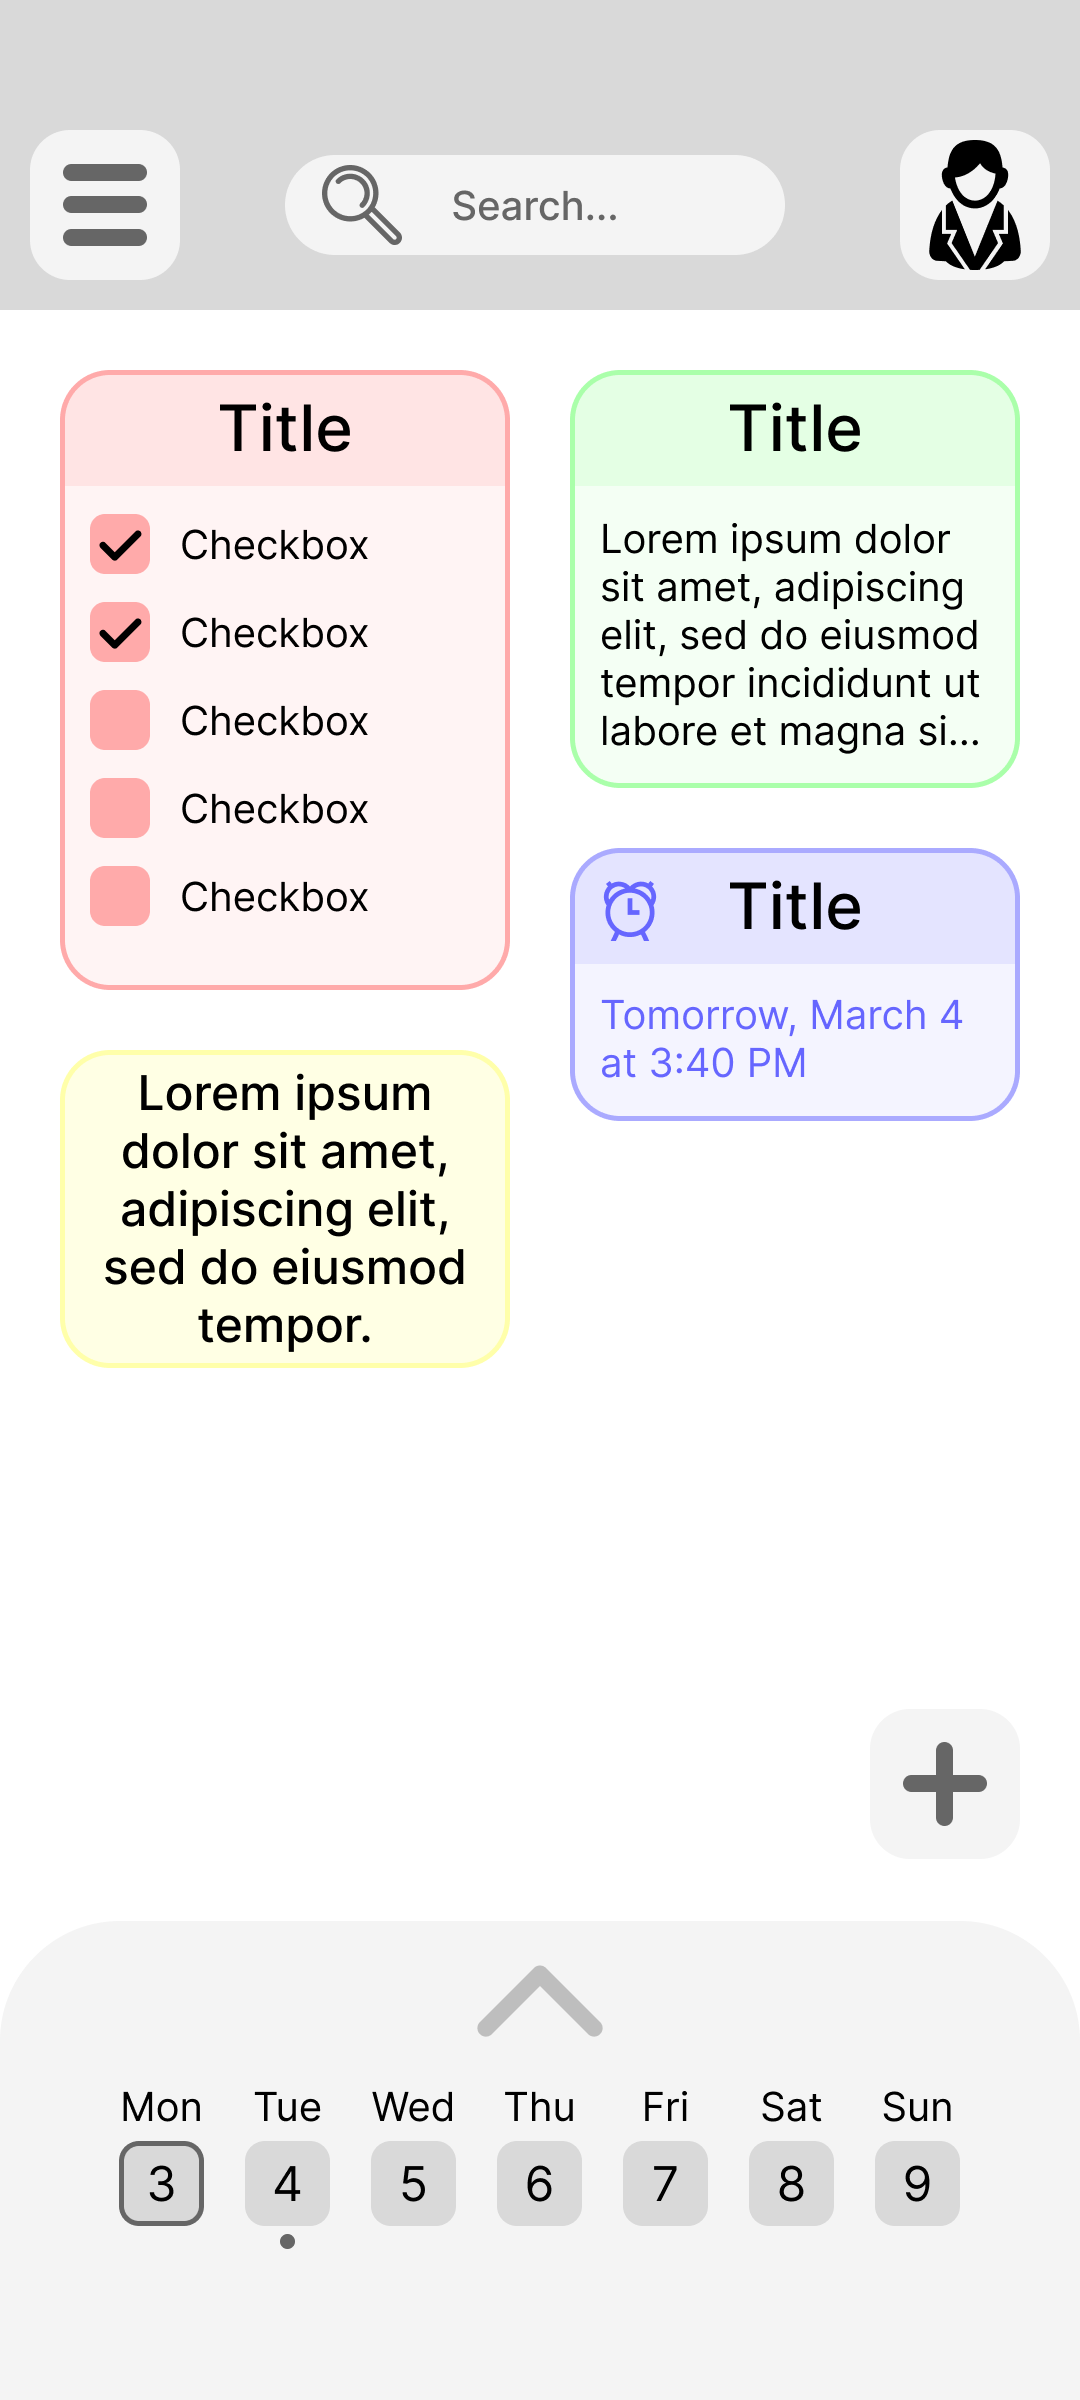
\includegraphics[scale=0.12]{Frame 1}
			\caption{Головний екран}
		\end{minipage}\hfill
		\begin{minipage}{0.48\textwidth}
			\centering
			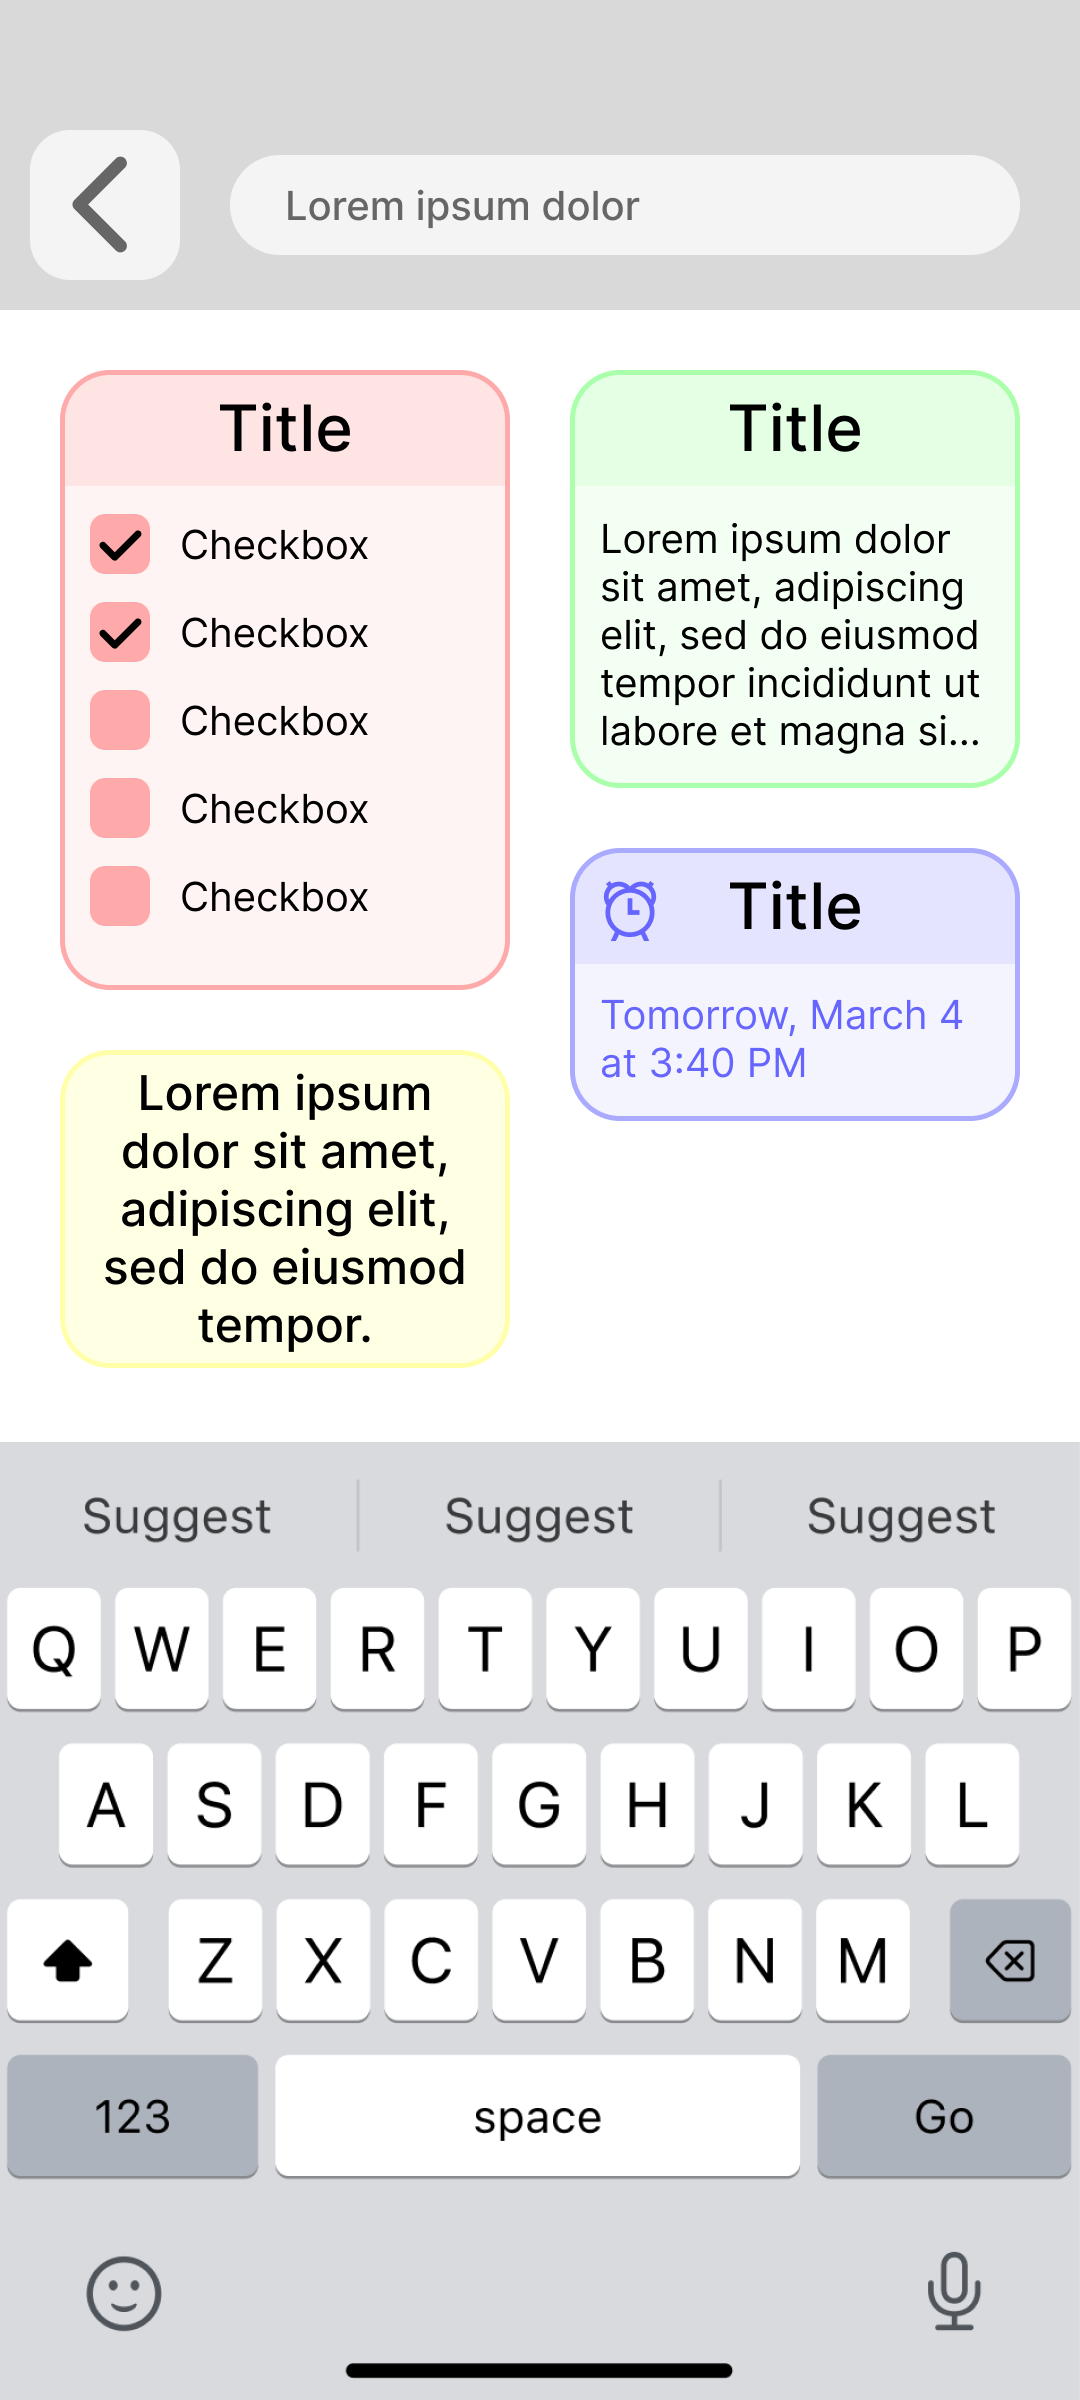
\includegraphics[scale=0.12]{Frame 2}
			\caption{Пошук серед нотаток}
		\end{minipage}
	\end{figure}
	
	\begin{figure}[H]
		\begin{minipage}{0.48\textwidth}
			\centering
			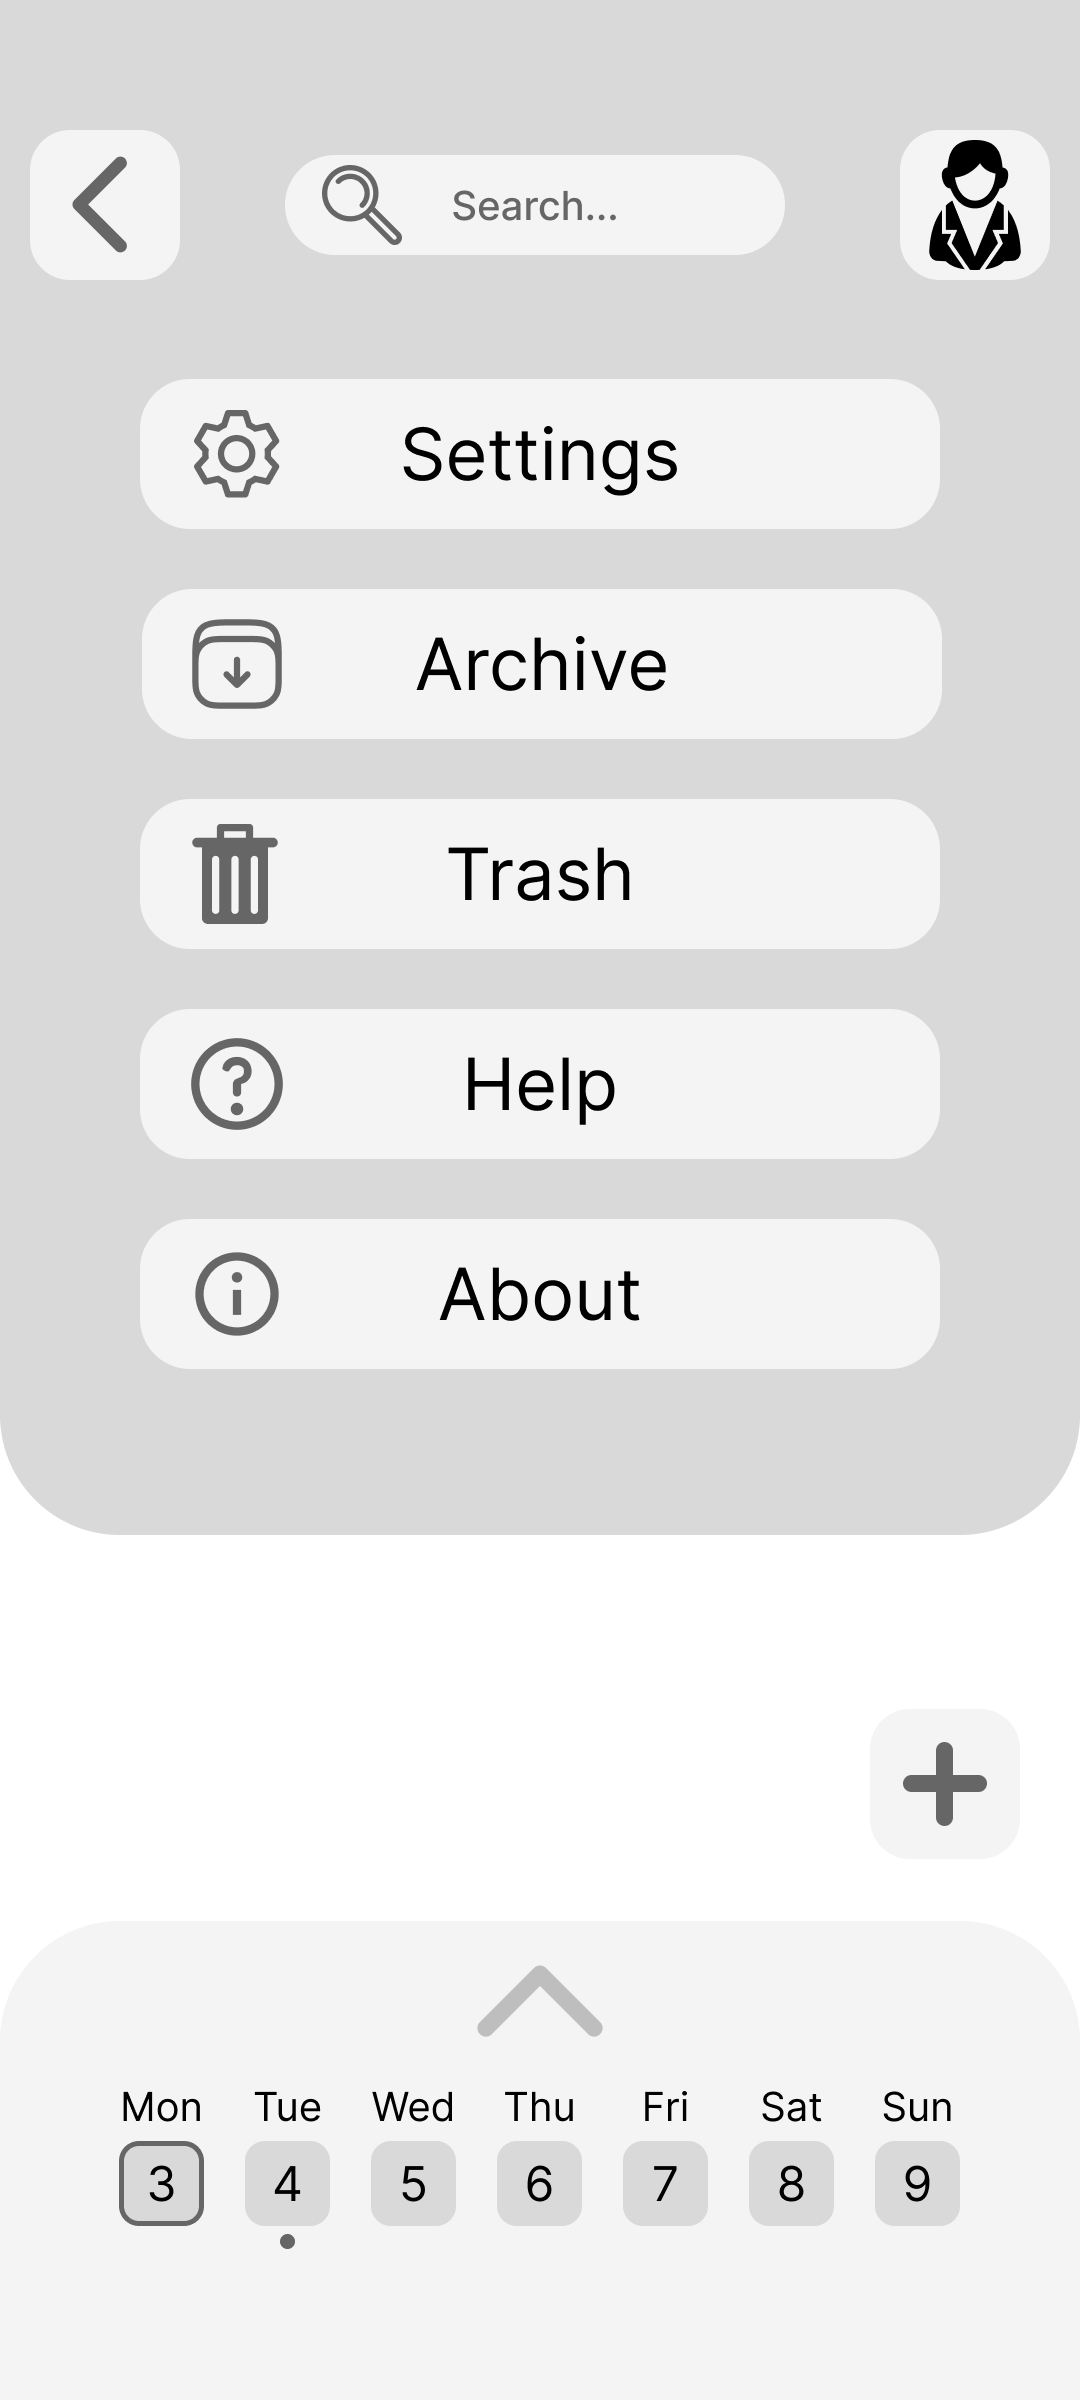
\includegraphics[scale=0.13]{Frame 3}
			\caption{Додаткове меню}
		\end{minipage}\hfill
		\begin{minipage}{0.48\textwidth}
			\centering
			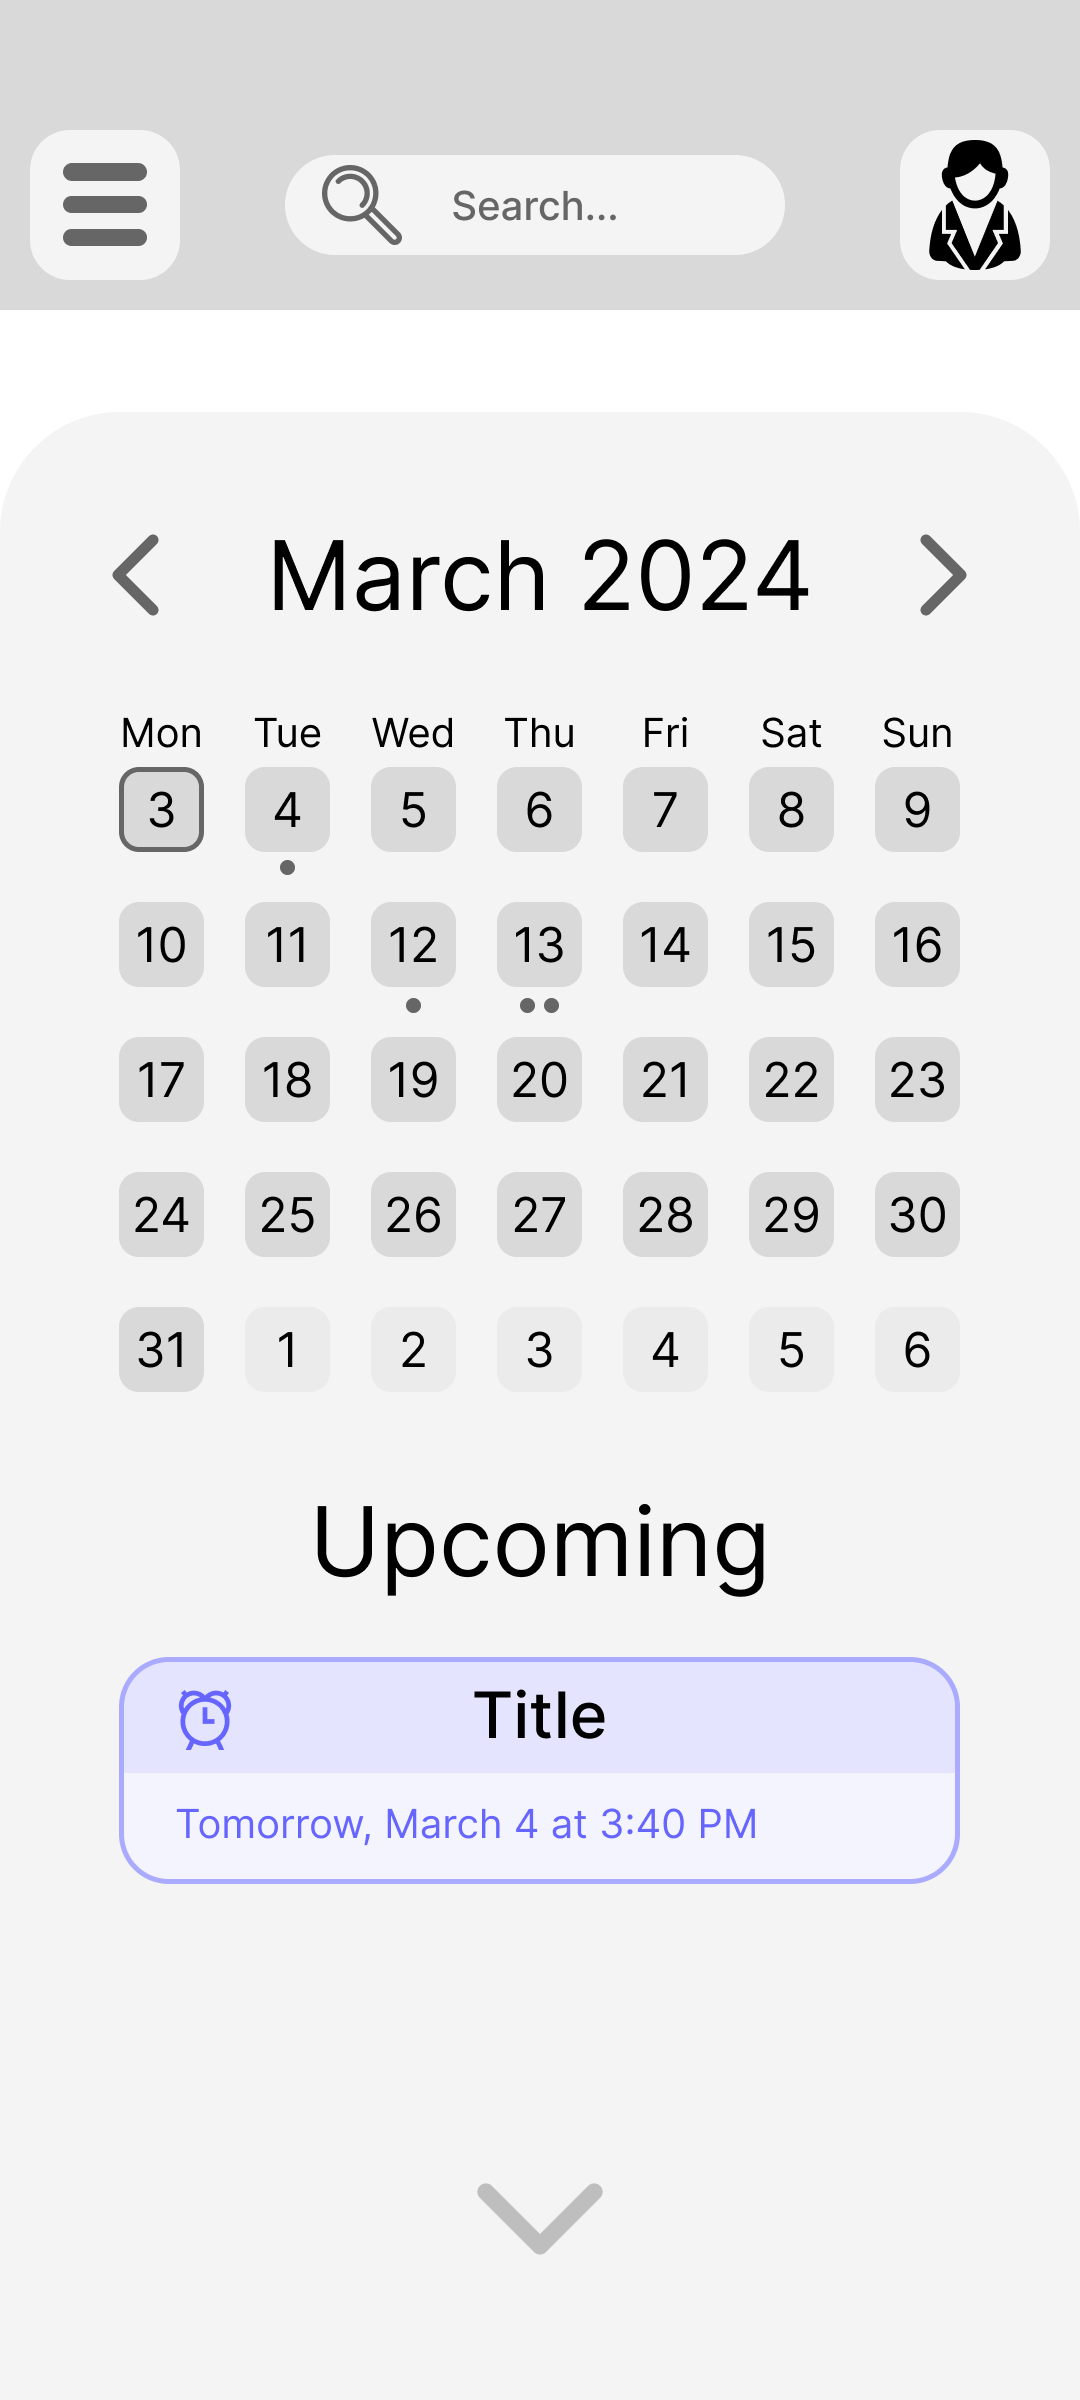
\includegraphics[scale=0.13]{Frame 4}
			\caption{Меню календаря}
		\end{minipage}
	\end{figure}
	
	\begin{figure}[H]
		\begin{minipage}{0.48\textwidth}
			\centering
			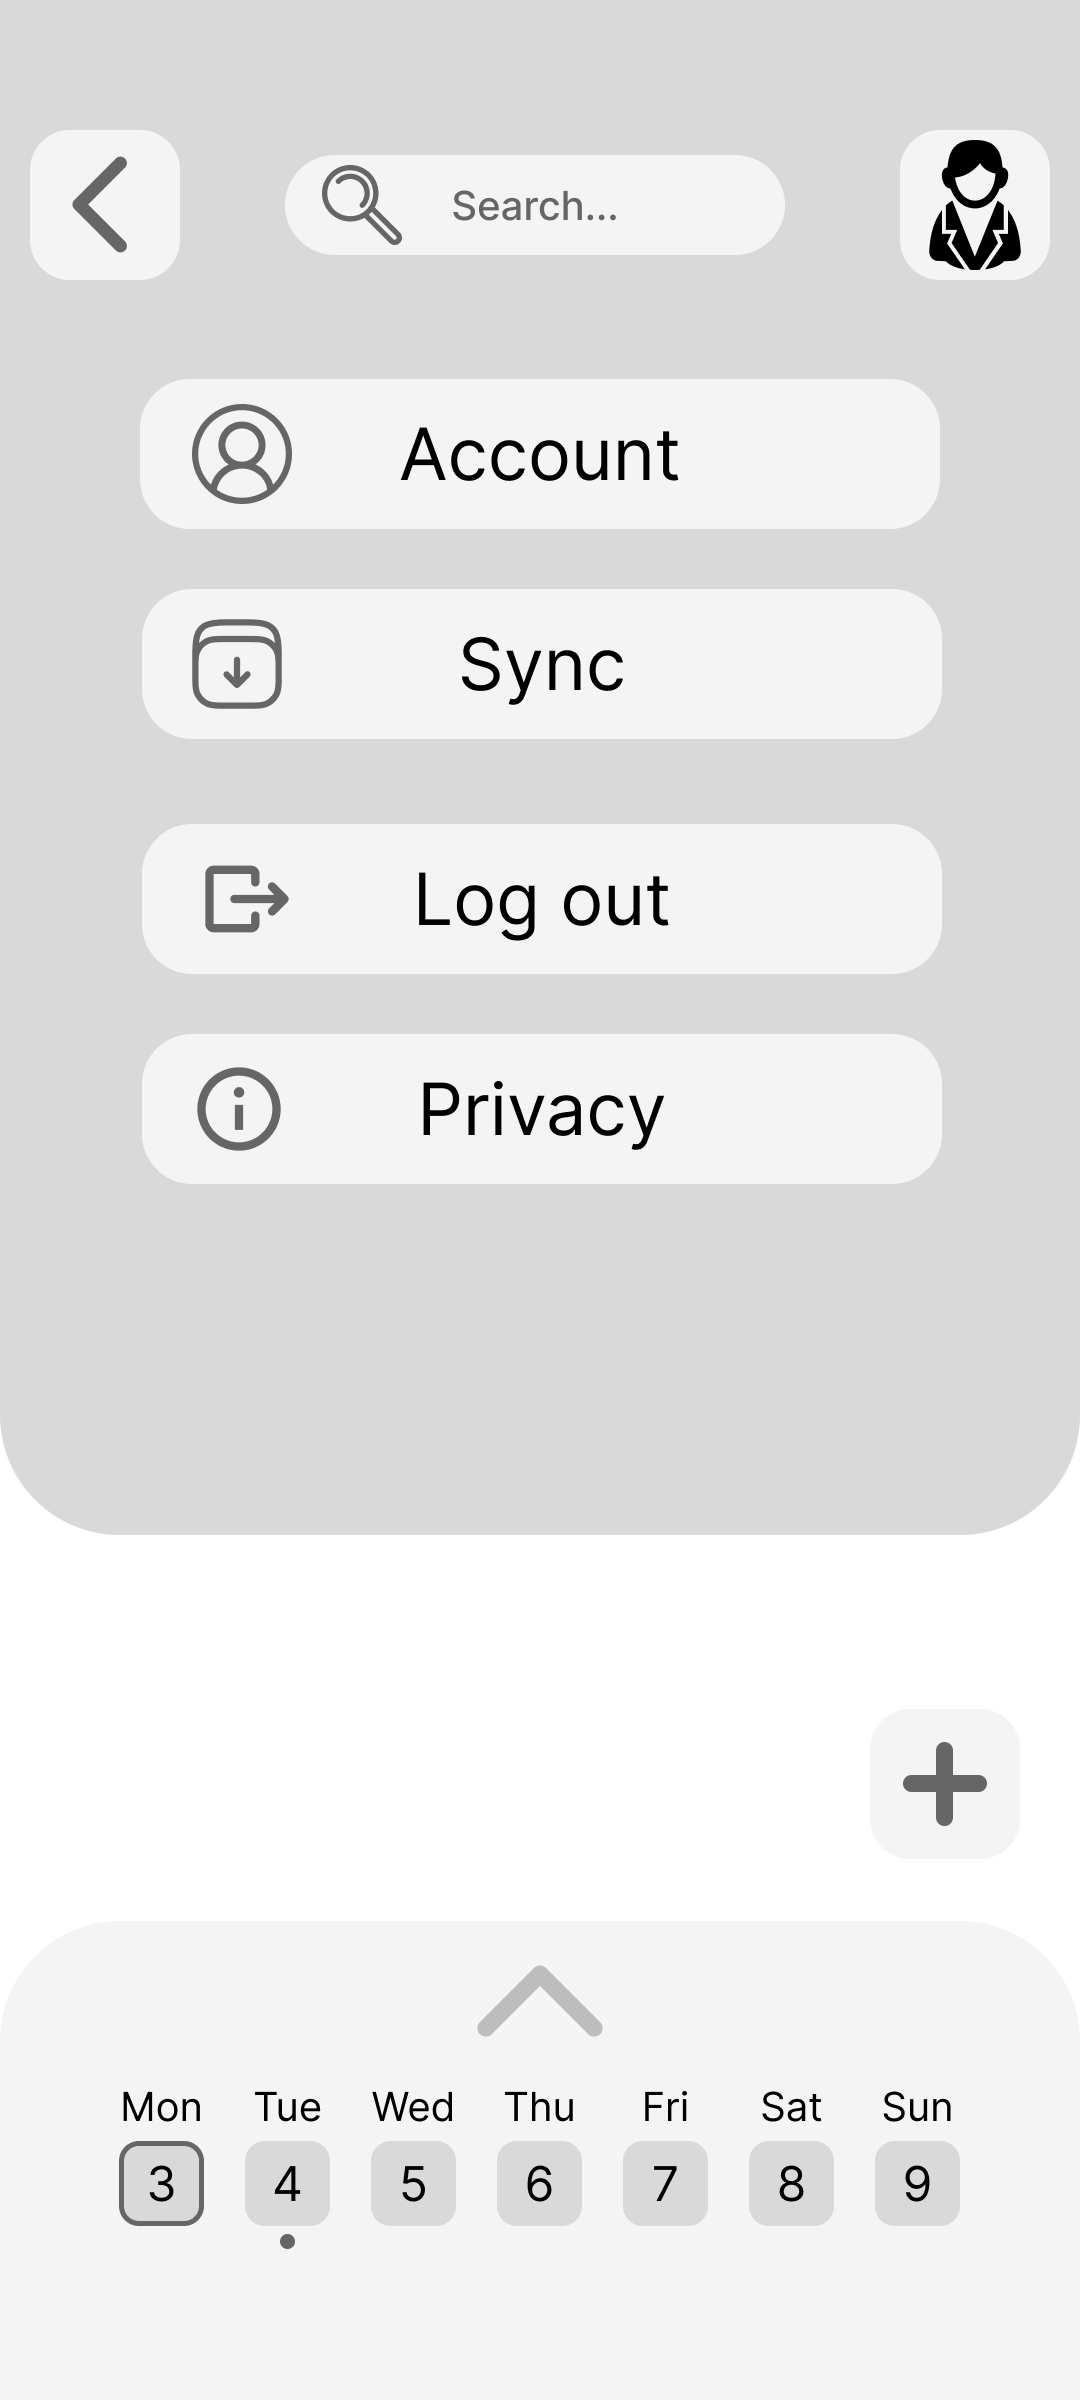
\includegraphics[scale=0.13]{Frame 5}
			\caption{Меню профілю користувача}
		\end{minipage}\hfill
		\begin{minipage}{0.48\textwidth}
			\centering
			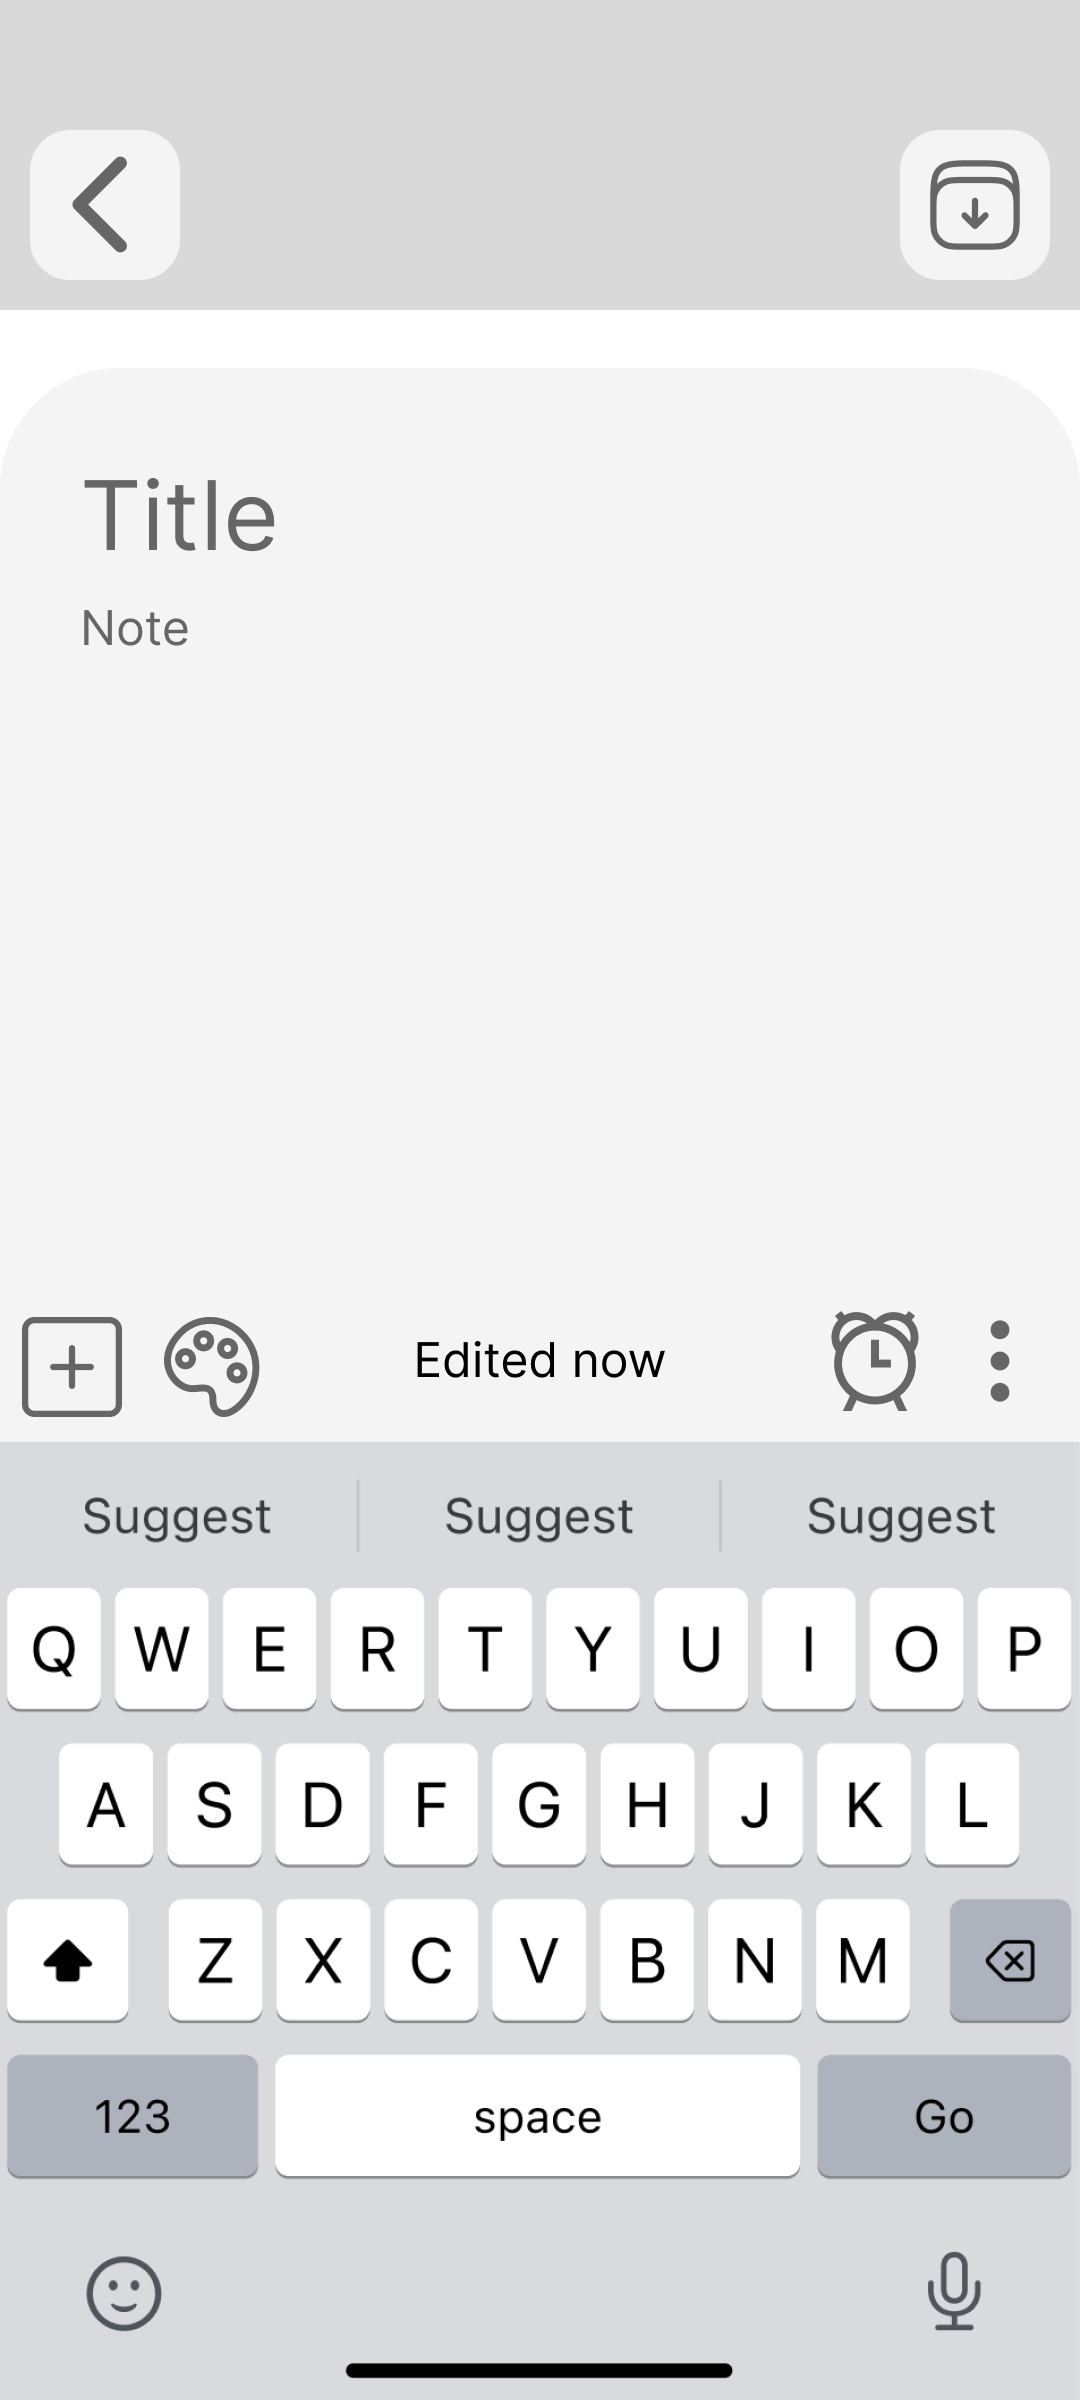
\includegraphics[scale=0.13]{Frame 6}
			\caption{Створення нотатки}
		\end{minipage}
	\end{figure}
	
	\begin{figure}[H]
		\begin{minipage}{0.48\textwidth}
			\centering
			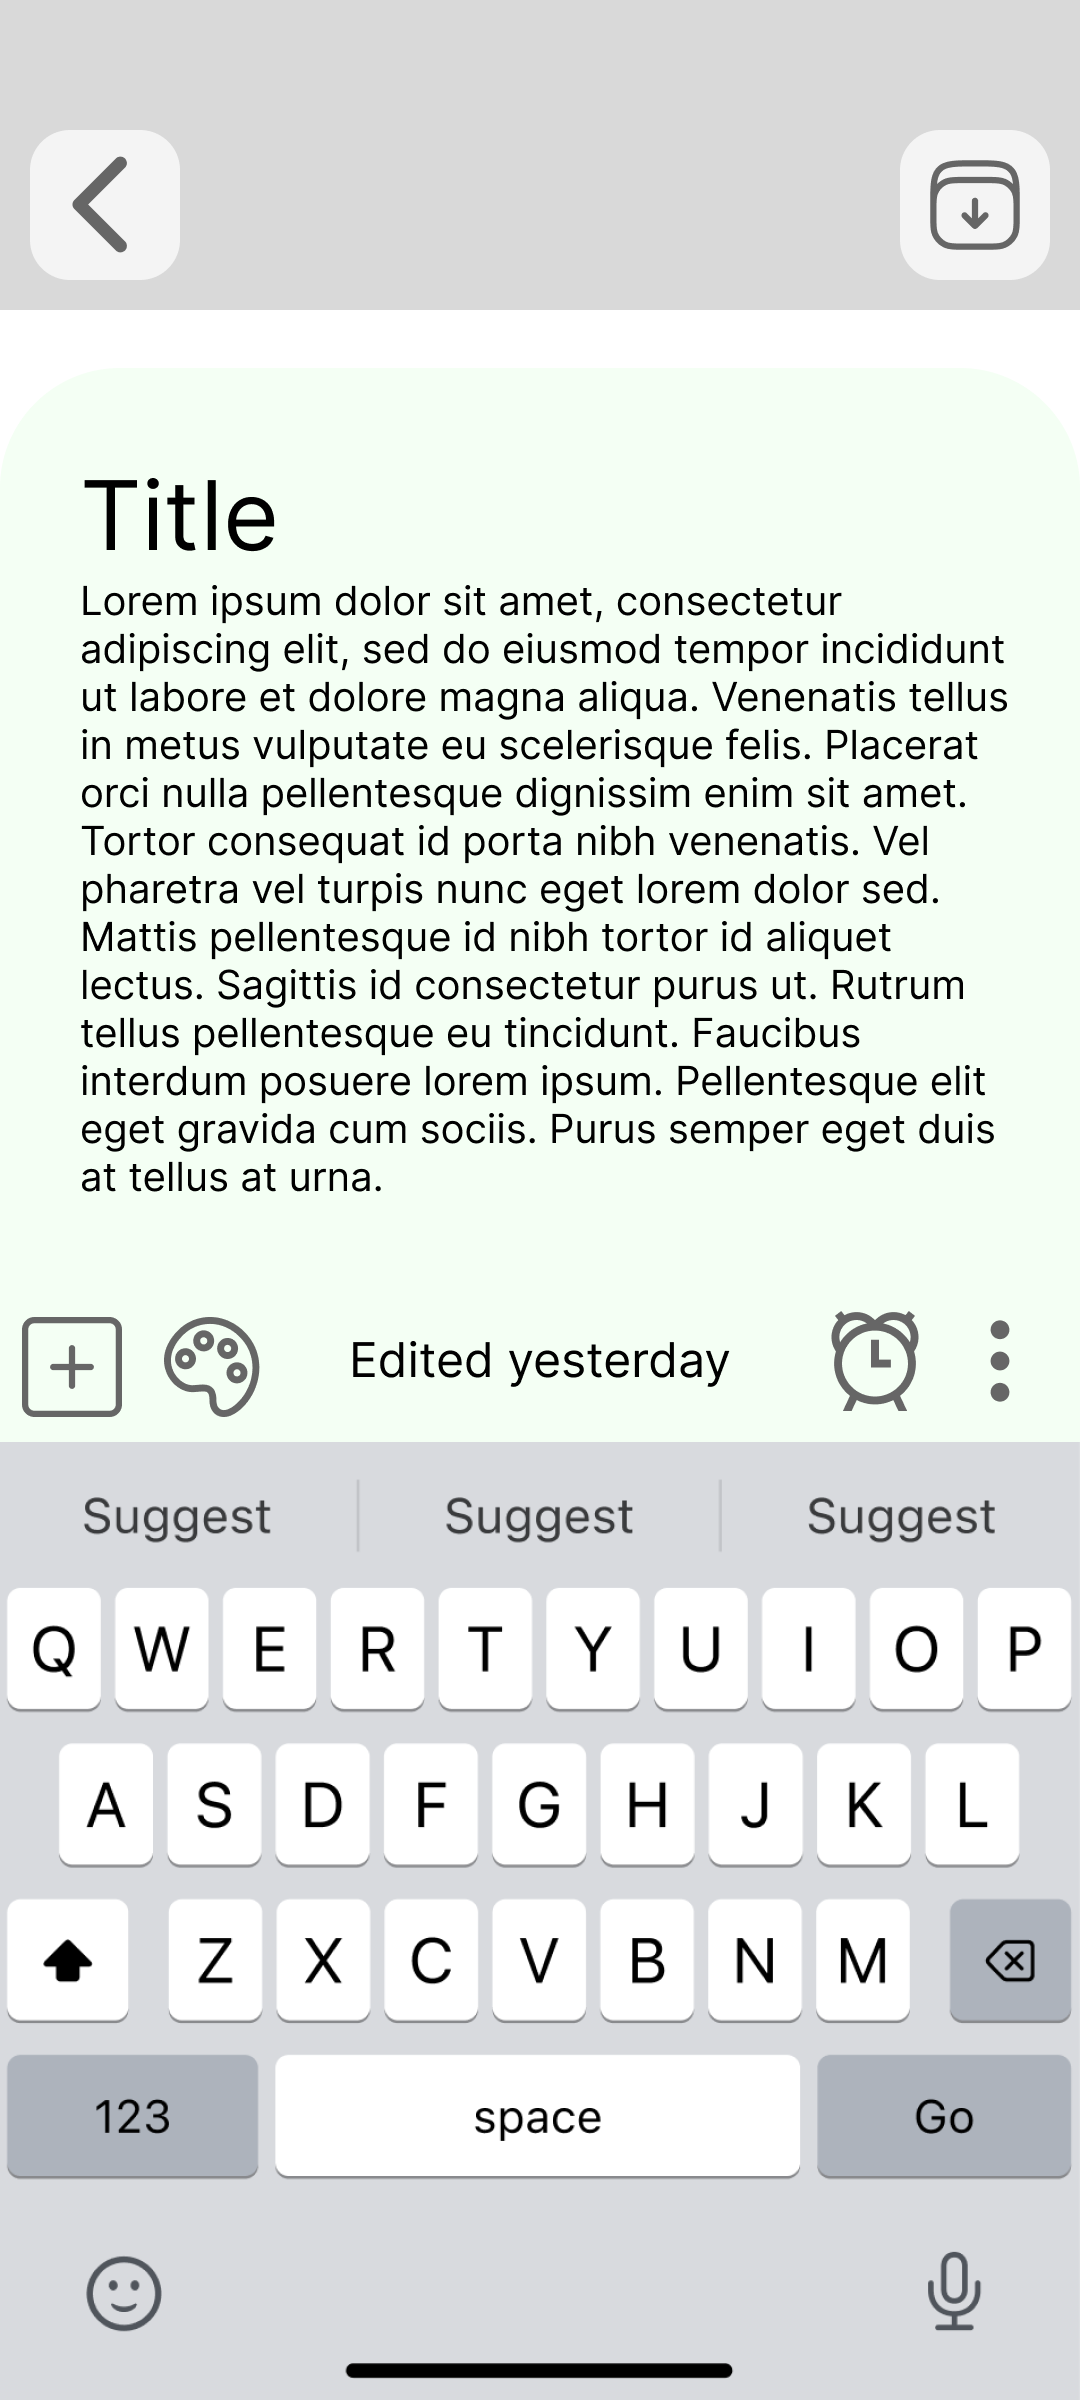
\includegraphics[scale=0.13]{Frame 7}
			\caption{Редагування нотатки}
		\end{minipage}\hfill
		\begin{minipage}{0.48\textwidth}
			\centering
			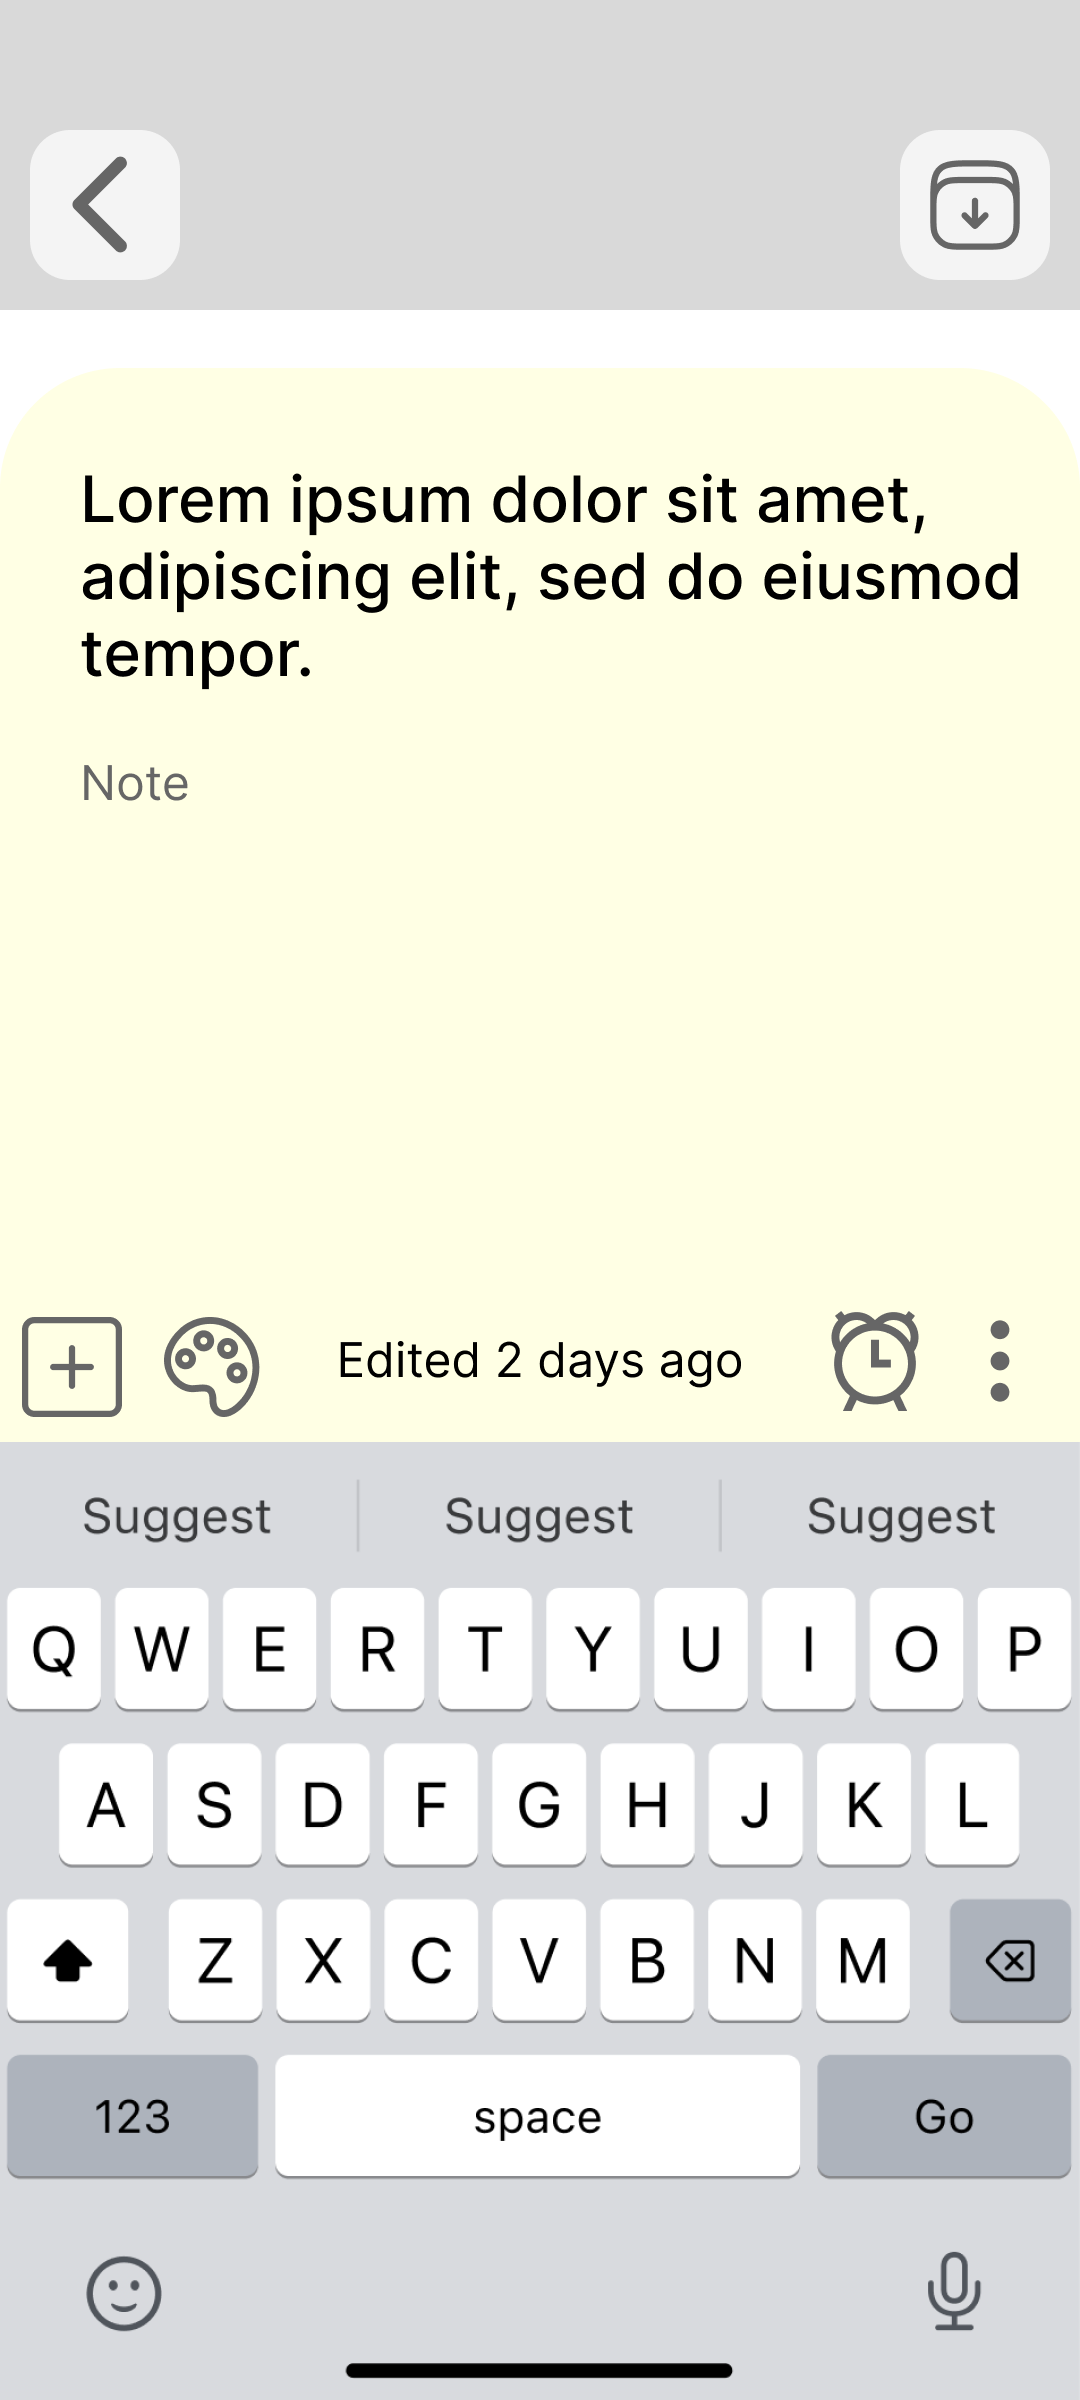
\includegraphics[scale=0.13]{Frame 8}
			\caption{Редагування нотатки}
		\end{minipage}
	\end{figure}
	
	\begin{figure}[H]
		\begin{minipage}{0.48\textwidth}
			\centering
			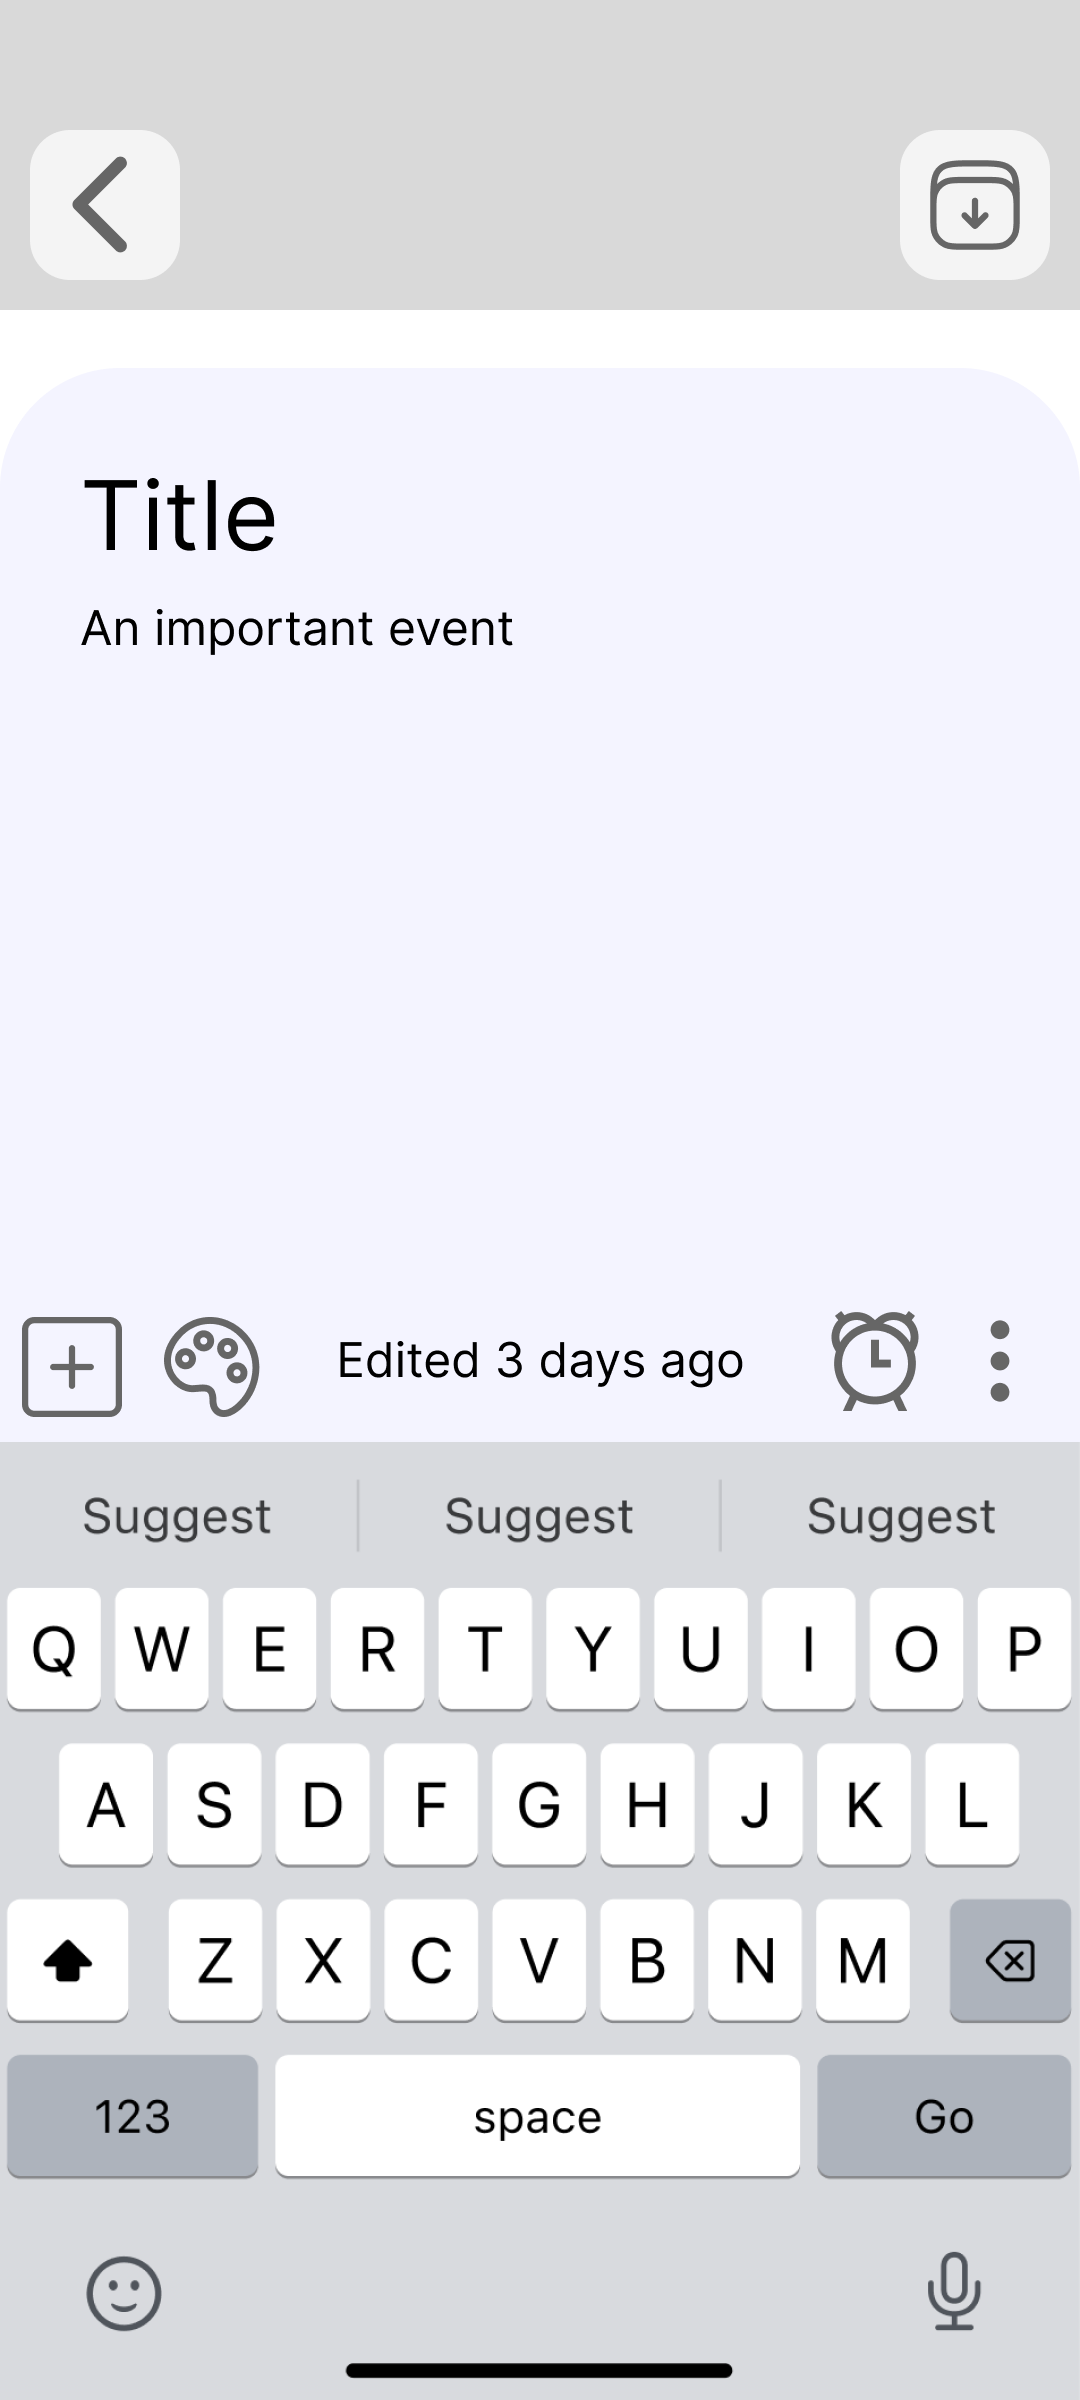
\includegraphics[scale=0.13]{Frame 9}
			\caption{Редагування нотатки}
		\end{minipage}\hfill
		\begin{minipage}{0.48\textwidth}
			\centering
			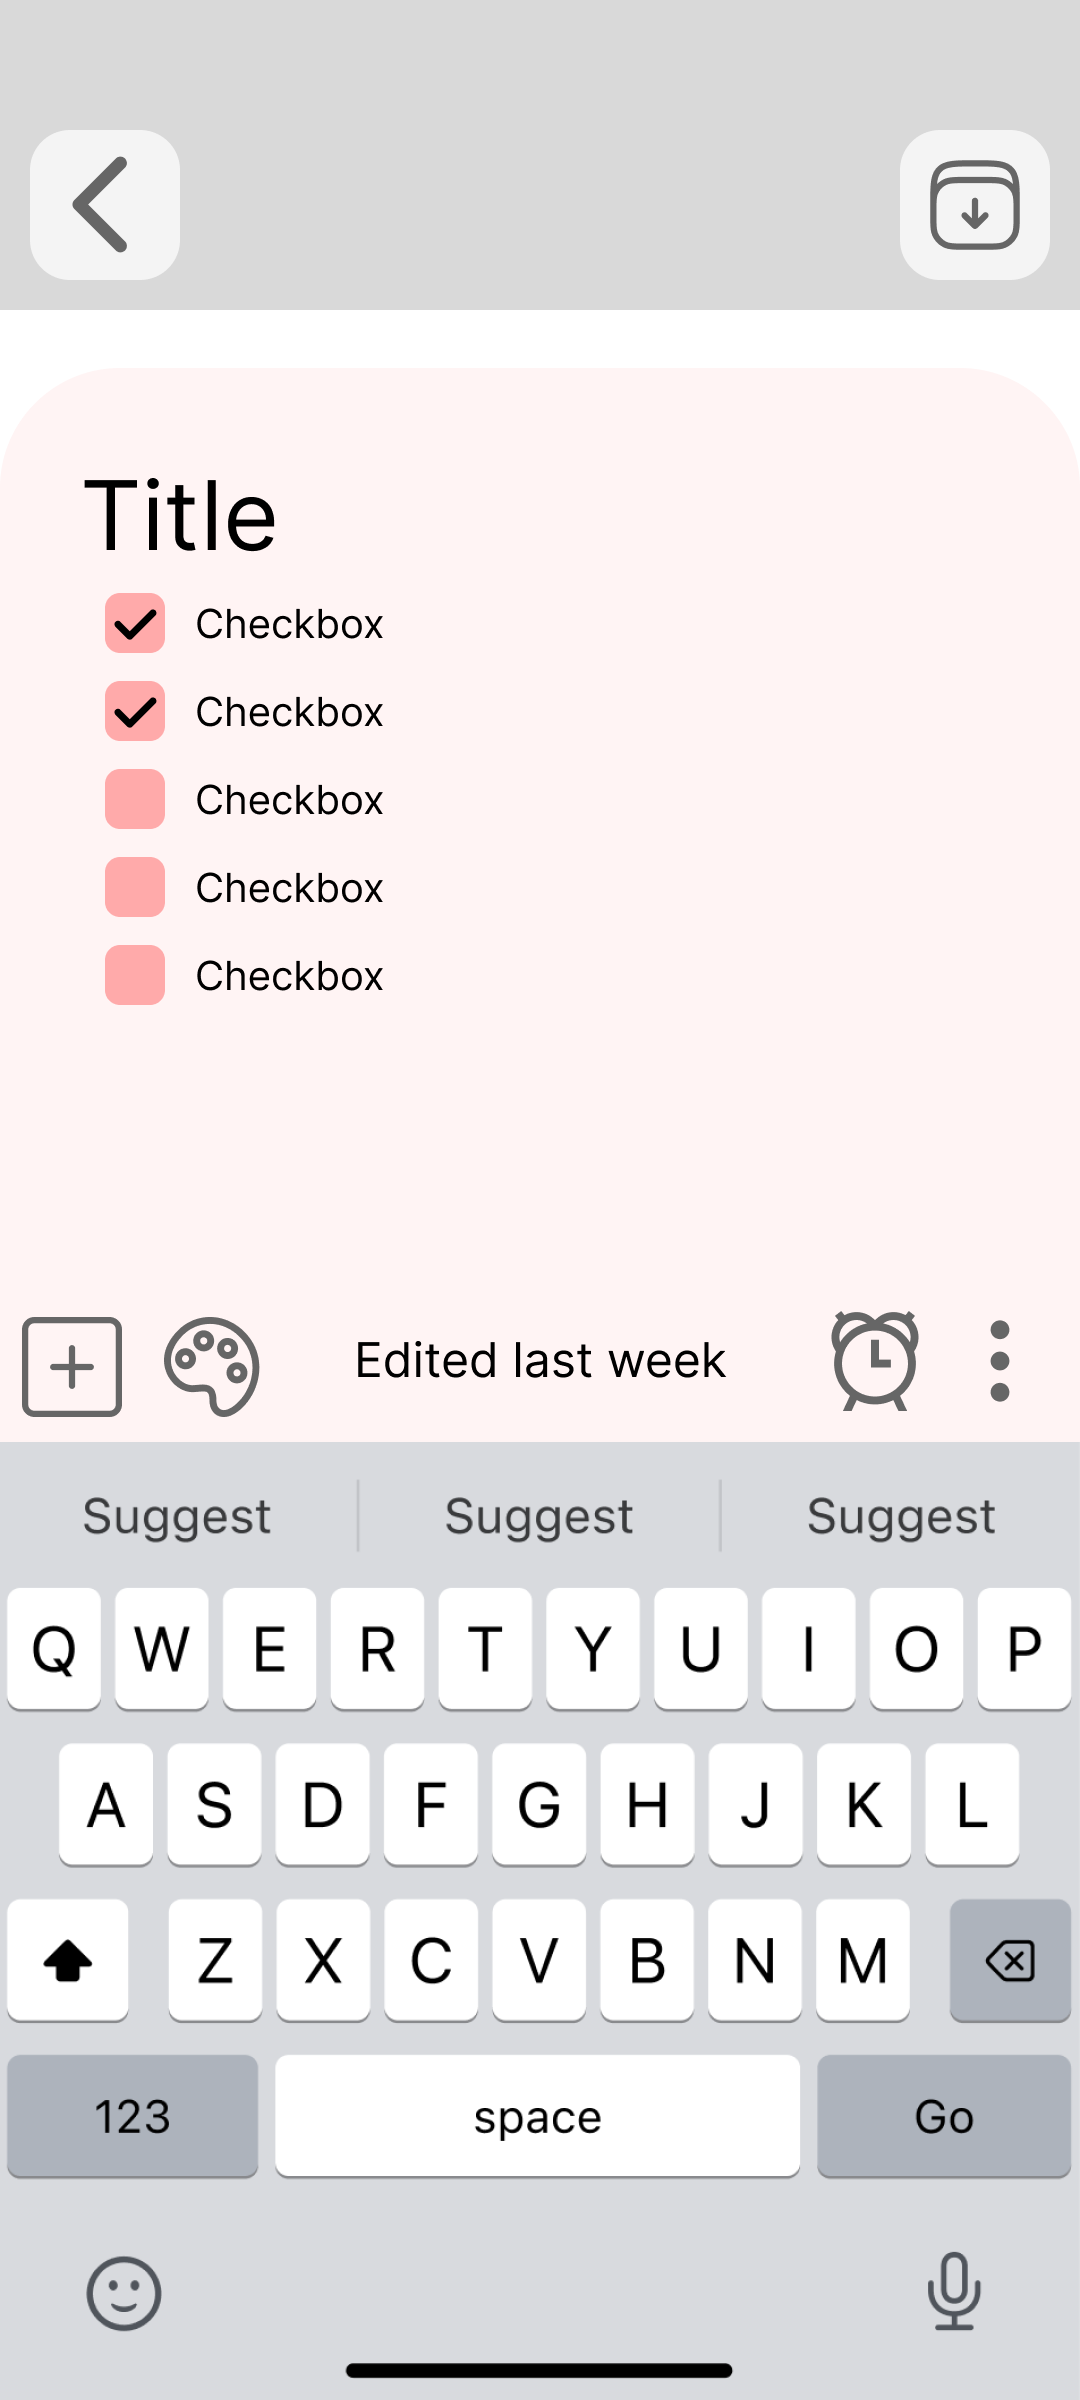
\includegraphics[scale=0.13]{Frame 10}
			\caption{Редагування нотатки}
		\end{minipage}
	\end{figure}
	
	\section*{Висновки}
	Під час виконання лабораторної роботи я спроектував інтерфейс користувача мобільного застосунку.
	    
\end{normalsize}
\end{document}
